%!TEX root = ../main_article.tex

\section{Experiment}
\label{sec:exp}

\subsection{Experiment Setting}
\noindent\textbf{Dataset.} The dataset we used is the Code Search Net dataset~(\citealp{CodeSearchNet}) 
preprocessed by GraphCodeBERT~(\citealp{GraphCodeBERT}). 
The parameter of the dataset is given below. We remove the data of Ruby and Javascript, 
as they are much less than other data. 

\noindent\textbf{Baseline model.} We choose CodeBERT~(\citealp{CodeBERT}) as the baseline model. 
It plays an important role in extracting code and query features. 
It is the encoder that first embed a code snippet or a natural query into a high-dimensional vector. 

\noindent\textbf{Disentangle network.} We use multiple linear perceptron as the basic 
layers of the network. We use ReLU~(\citealp{agarap2018deep}) as the activation. 

\noindent\textbf{Training setting.} We use an RTX 3090 GPU for training. 
The batch size of the training procedure is 128. The total training epoch number is 3. 
We use the package of Transformers 4.24.0 and Pytorch 1.12.0, based on Python 3.8.13.

\begin{figure}[htb]
	\centering
	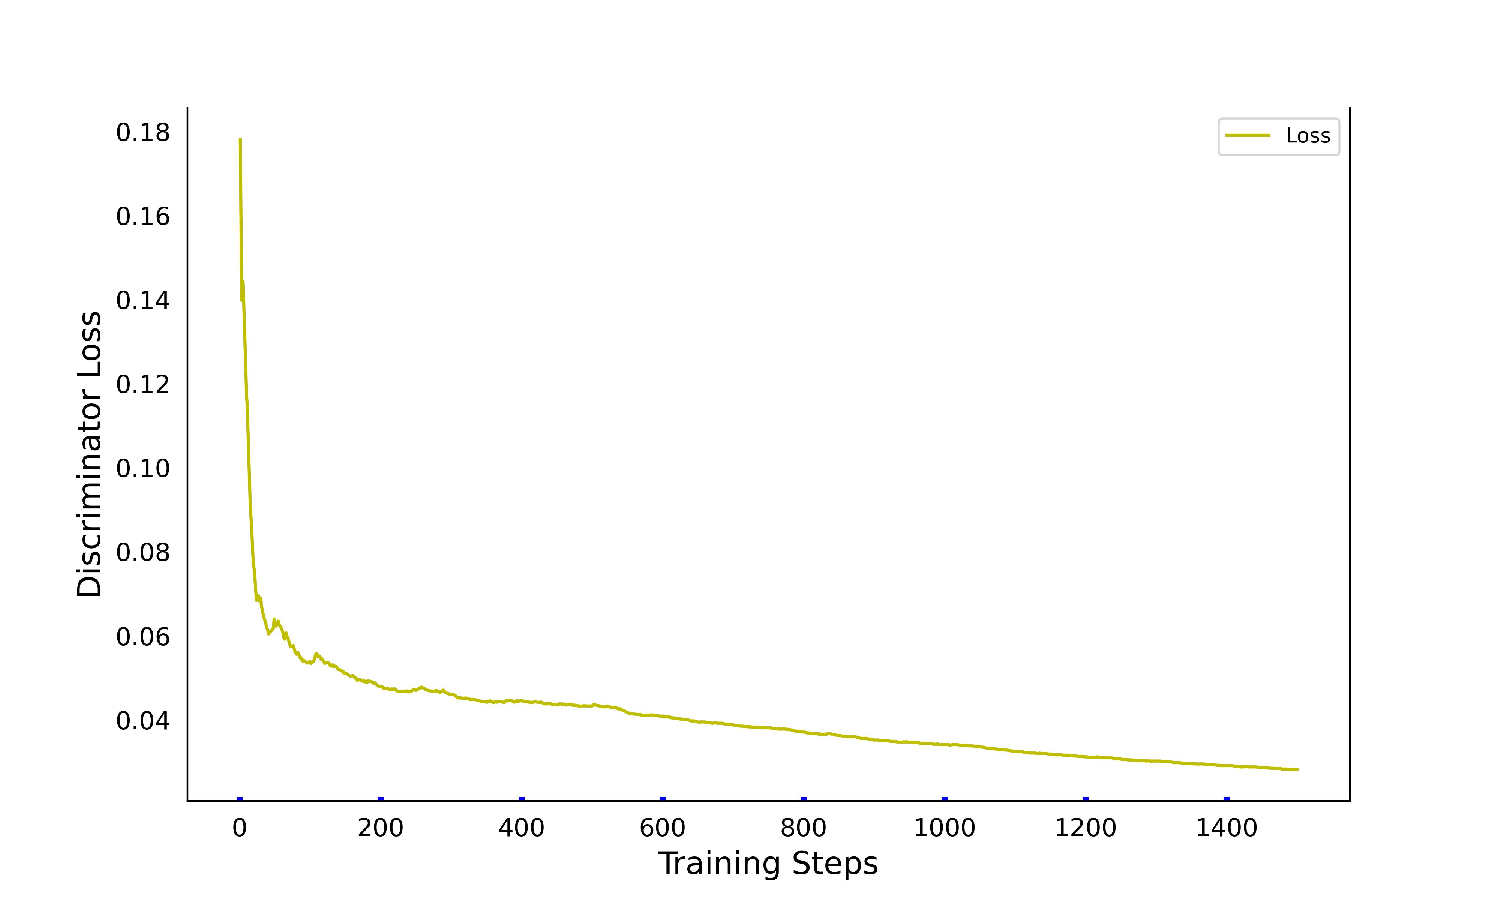
\includegraphics[width=0.8\linewidth]{imgs/discri_loss.pdf}
	% \vspace{-15pt}
	\caption{Loss change of discirminator during training.}
	% \vspace{-12pt}
	\label{fig:disloss}
\end{figure}

\subsection{Analysing Training Process} 
\subsubsection{Disentangle Network 1.}
We illustrated the change of discriminator loss during training in Fig~\ref{fig:disloss}. 
It is obviously that the loss of the discriminator is able to converge, 
while there is still slightly increment in some period, e.g., step 50 and step 100.
Fig~\ref{fig:genloss} shows the loss change of the generator during training. 
There might be overfitting, 
as the loss first decreases and then rises with increasing iterations.


\begin{figure}[htb]
	\centering
	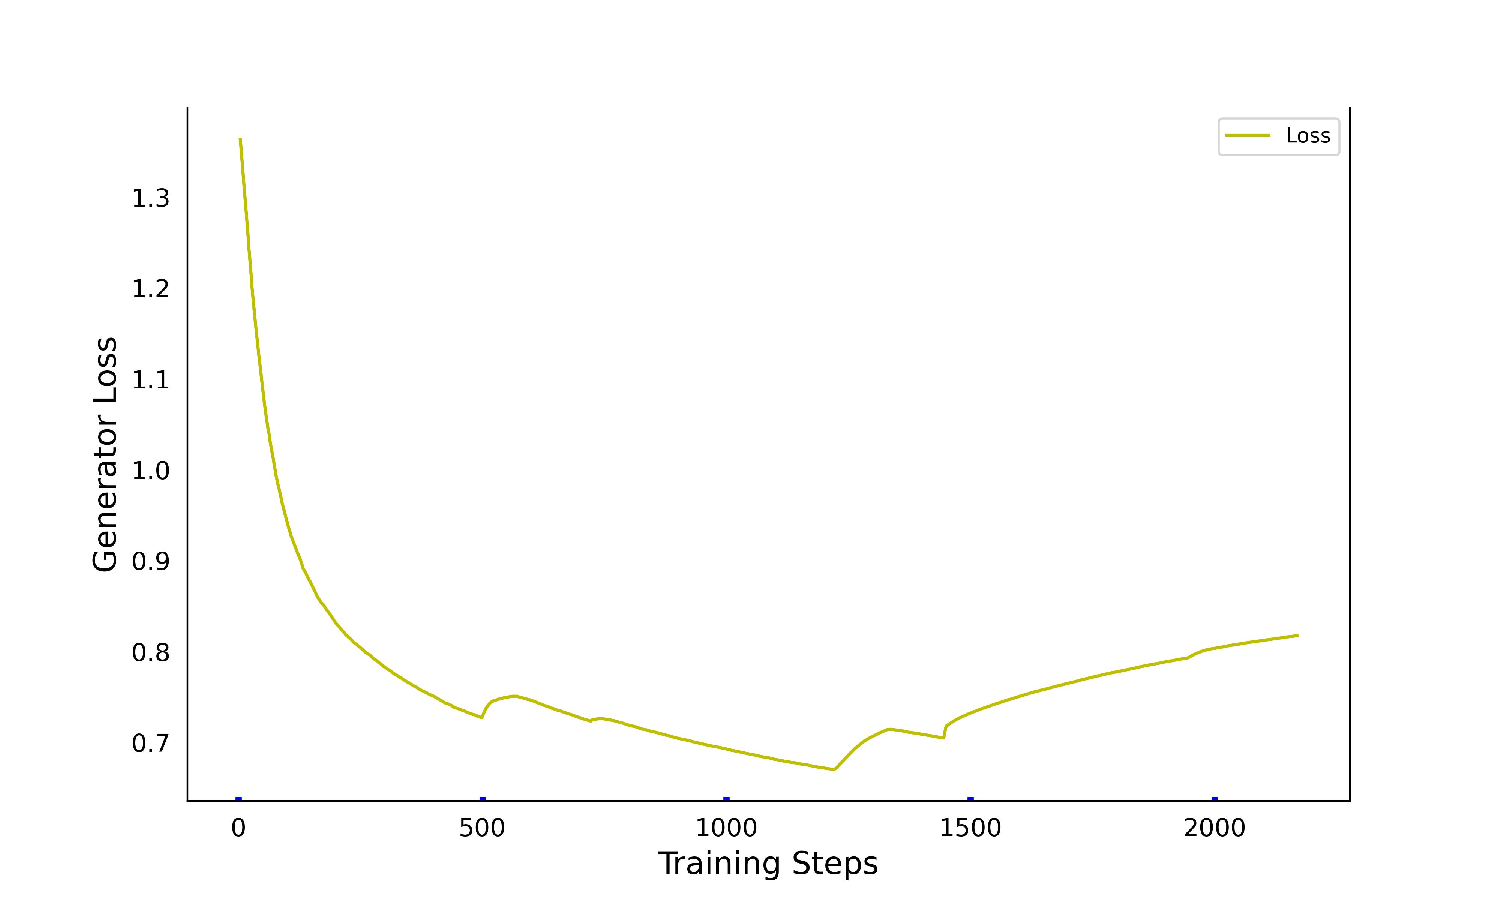
\includegraphics[width=0.8\linewidth]{imgs/gen_loss.pdf}
	% \vspace{-15pt}
	\caption{Loss change of generator during training.}
	% \vspace{-12pt}
	\label{fig:genloss}
\end{figure}

\begin{figure}[htb]
	\centering
	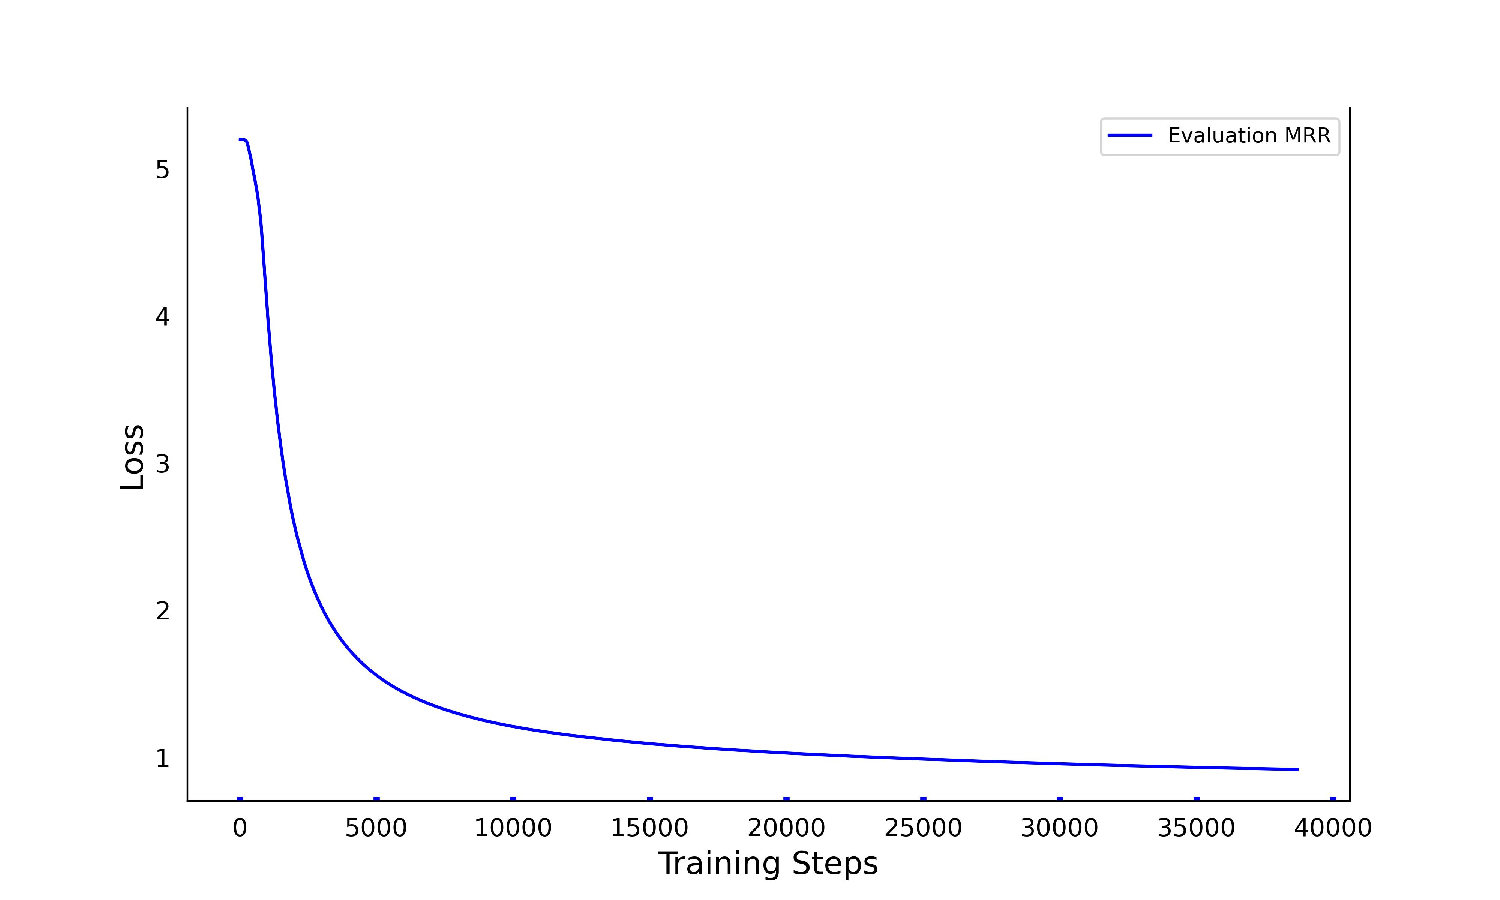
\includegraphics[width=0.8\linewidth]{imgs/st2_loss.pdf}
	% \vspace{-15pt}
	\caption{Loss of network 2 during training.}
	% \vspace{-12pt}
	\label{fig:st2loss}
\end{figure}

\subsubsection{Disentangle Network 2.}
We list hybrid loss change of network based on strategy 2 in Fig~\ref{fig:st2loss}. 
It is apparent the loss is decreasing and able to converge. 
Fig~\ref{fig:st2eval} represents the evaluation index change in the training period, 
using MRR, which is shown in Eq~\ref{MRR}, as the index and with the evaluation step of 2, 000. 

\begin{figure}[htb]
	\centering
	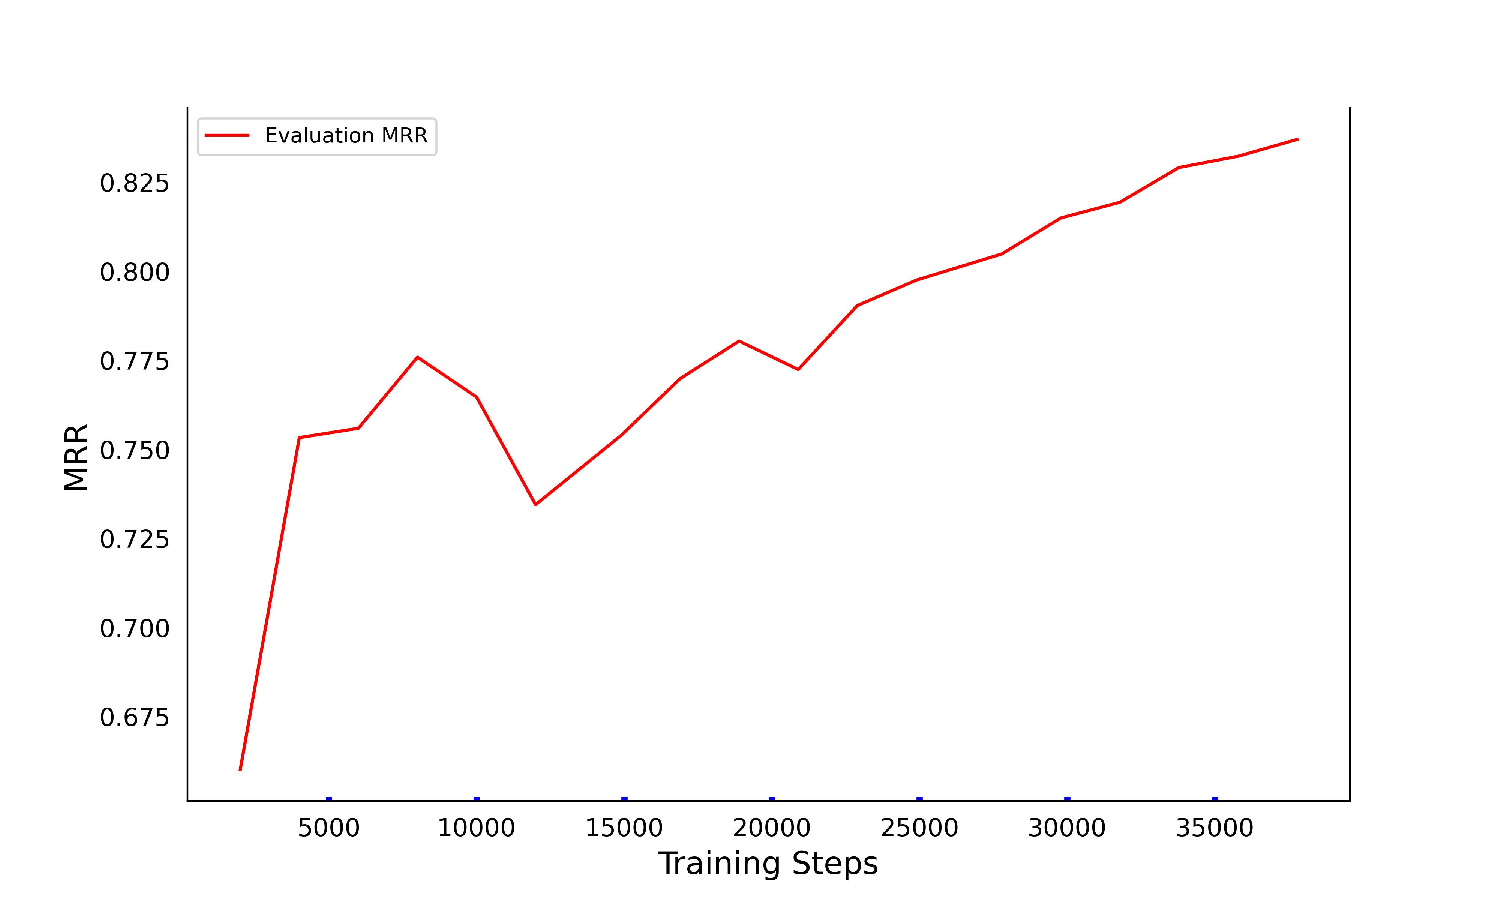
\includegraphics[width=0.8\linewidth]{imgs/st2_eval.pdf}
	% \vspace{-15pt}
	\caption{MRR change in evaluation during training.}
	% \vspace{-12pt}
	\label{fig:st2eval}
\end{figure}

\subsection{Analysing Embedding Vectors after Disentangling}
Intuitively, identity and semantic information can be divided easily after 
applying the disentangle strategy we proposed. Thus, we first use t-SNE~\cite{tSNE}, 
which is a dimensionality reduction method, to 
reduce high-dimensional vectors to 2 dimensions. 
Then we visualize the 2-dimensional vectors. 
We sample 5, 000 code snippets from the whole dataset. 
And then draw the embedding graph. For the strategy 1 network, 
we visualize the vectors output by the origin CodeBERT and the generator. 
For the strategy 1, we illustrate embedding vectors output 
by CodeBERT and disentangle network in Fig~\ref{fig:st2_gan}. Compared to the CodeBERT vectors, i.e., 
blue points, the generator output, i.e., yellow points, 
is less concentrated in the same area. For the strategy 2, 
we visualize v1 and v2 vector, which is considered have identity and semantic information, 
respectively. From the graph~\ref{fig:st2_emb} we can see that, 
two types of the vectors can basically be separated. 

\begin{figure}[htb]
	\centering
	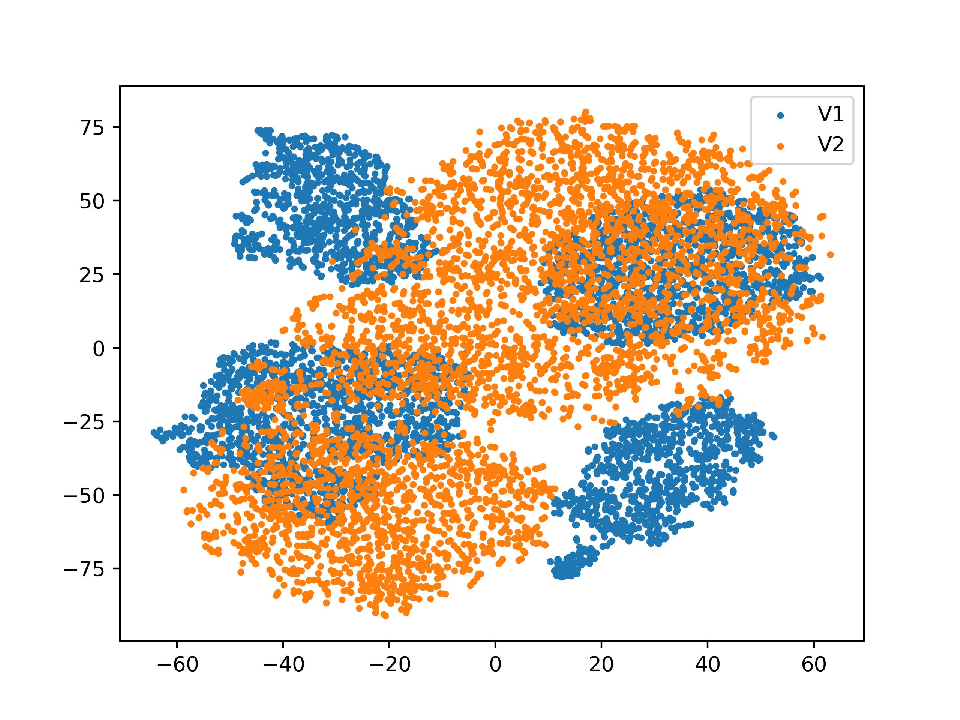
\includegraphics[width=0.9\linewidth]{imgs/st2_emb.pdf}
	% \vspace{-15pt}
	\caption{Embedding vector comparision of strategy 2 network.}
	% \vspace{-12pt}
	\label{fig:st2_emb}
\end{figure}

\begin{figure}[htb]
	\centering
	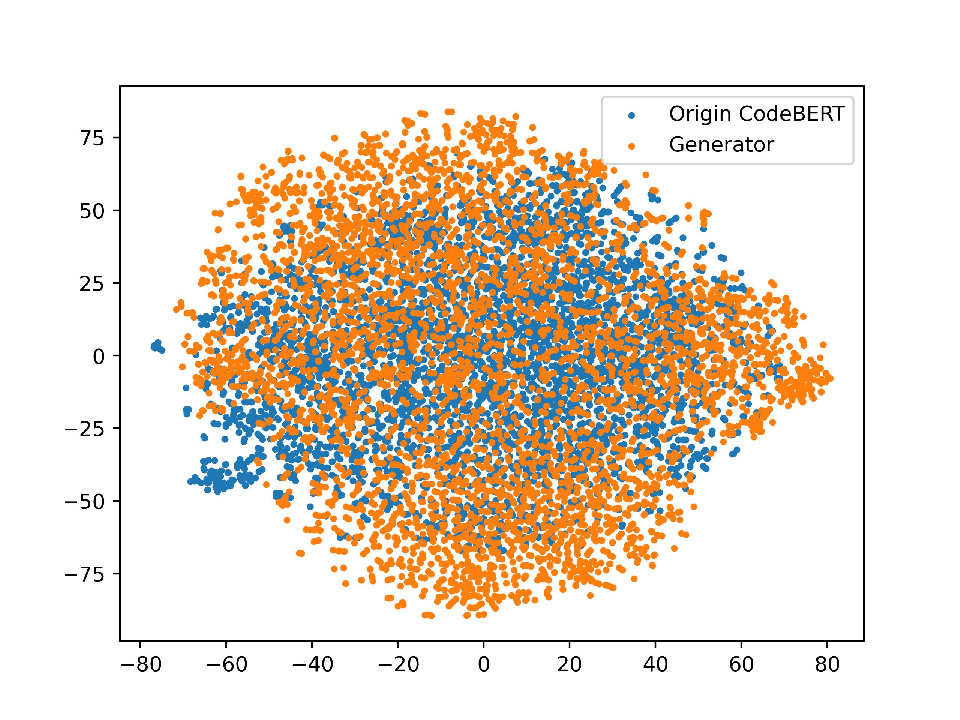
\includegraphics[width=0.9\linewidth]{imgs/gan_emb.pdf}
	% \vspace{-15pt}
	\caption{Embedding vector comparision of strategy 1 network.}
	% \vspace{-12pt}
	\label{fig:st2_gan}
\end{figure}

\subsection{Analysing Code Search Results}
In this section, 
we try to figure out the code search performance of two disentangle networks. 
We use MRR as the evaluation indicator, 
which is the reciprocal of the correct result among all returned results 
and it is given as Eq~\ref{MRR}, where $Q$ is the total test number and $rank_i$ represents the correct rank among all results..

\begin{equation}\label{MRR}
	MRR = \frac{1}{Q} \sum_{i=1}^Q \frac{1}{rank_i}
\end{equation}

% Table generated by Excel2LaTeX from sheet 'Sheet1'
\begin{table}[htbp]
	\centering
	\caption{MRR Comparisions}
	\begin{tabular}{ccc}
	\toprule
	& Strategy 1 & Strategy 2 \\
	\midrule
	Python & 0.597 & 0.601 \\
	Go  & 0.873 & 0.882 \\
	Java & 0.712 & 0.703 \\
	Php & 0.684 & 0.673 \\
	\bottomrule
	\end{tabular}%
	\label{tab:mrr_comparision}%
\end{table}%

Table 1 shows the code search MRR results. 
The left first column indicates the language of data. 
The top row indicates the strategy we proposed. 
From the results we can see that there is a small performance increment in Python, 
compared to the original results in~\ref{section:1}, 
while a slightly decrease occurs in other languages.
It is clear that strategy 1 and strategy 2 can reach a similar result, 
while Java and Php data have a better MRR in strategy 1, 
and Python and Go data are better in strategy 2.

\section{Discussion and Conclusion}
In this paper, we propose two disentangle strategies 
for tackling performance decline when fine-tuning CodeBERT 
for the code search task with multiple language data. 
In strategy 1, we leverage a GAN-based model, to eliminate identity information. 
In strategy 2, we use MLPs to divide embeddings by maximize their KL divergence. 
Experiments show our work achieve some results. 

However, we only consider identity information as the signal that 
distinguish program languages from each other, e.g., a classification task. 
Whether the identity information is equal to syntax information, 
needs more experiments to proof. Besides, the code search performance 
still have room for improvement. We hope our work can be reference for 
the same field researchers.
